\label{sec:methods}
\section{Problemstellung und Methoden}

Das Problem ist, im zweidimensionalen Raum realistische Schatten zu berechnen, die wie echte
Schatten aus den drei Teilen "`Umbra"', "`Penumbra"' und "`Antumbra"'.
Also keine harten Schatten wie bei einem Punktlicht, sondern weiche Schatten und auch
Überlagerungen von Schatten.

\begin{figure}[t]
	\centering
	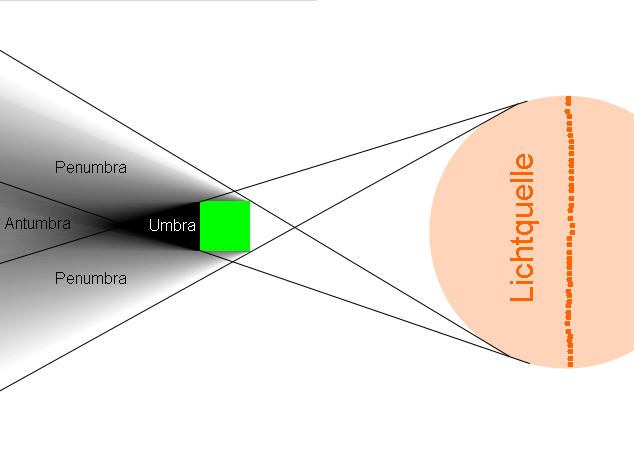
\includegraphics[width=\columnwidth]{images/umbra_penumbra_antumbra.png}
	\caption{Umbra, Penumbra \& Antumbra}
	\label{fig:umbra}
\end{figure}

\subsection{Umbra, Penumbra und Antumbra}

In der Theorie von Schatten wird ein Schatten in 4 Teile zerlegen (Abbildung \ref{fig:umbra}).
\begin{enumerate}
 \item \emph{Umbra}, der Kernschatten, ist der Teil des Schattens der von keinerlei Licht erreicht wird.
       Wenn es nur eine Lichtquelle gibt, dann hat jeder Schatten einen Umbra.
 \item \emph{Antumbra}, der weiche Schatten, der hinter dem Umbra entsteht. Dieser Bereich entsteht nur,
       wenn die Lichtquelle größer ist, als das Objekt, das den Schatten wirft. Der Antumbra beginnt an
       dem Punkt, an dem das Objekt die Lichtquelle nicht mehr vollständig verdecken kann und man die
       Ränder der Lichtquelle sehen kann.
 \item \emph{Penumbra}, die zwei weichen Schatten, die an den Seiten des Umbras entstehen. Diesen Bereich
       gibt es immer, wenn der Schatten nicht von einer Punktlichtquelle geworfen wird, in der realen
       Welt also immer. In diesem Bereich beginnt man die Seite der Lichtquelle zu sehen, die vorher im
       Umbra verdeckt wurde.
\end{enumerate}
Diese 3 separaten Bereiche eines Schatten sollten optisch realistisch dargestellt werden können.
Damit gilt also als Anforderung, dass Lichtquellen simuliert werden können, die eine Breite haben
und nicht einfach nur ein Punkt sind.


\subsection{Shadow Mapping}

Das "`Shadow Mapping"'-Verfahren, auch "`Projective shadowing"' genannt, berechnet eine sehr einfache,
aber dafür auch effiziente Annäherung für Schatten. Das Verfahren kann vollständig auf dem
Grafikprozessor ausgeführt werden, was nochmals zu einer Beschleunigung führt. Die Berechnung der
Szene wird dabei grob in die folgenden Schritte unterteilt:

\begin{enumerate}
 \item Als erstes wird die Szene von der Sicht des Lichts aus berechnet. Dabei wird für Punktlichter
       eine perspektivische Projektion verwendet, während für das Umgebungslicht (Sonnenlicht) eine
       orthografische Projektion verwendet wird.

       Beim berechnen der Szene in diesem Schritt werden Farben und Texturen in der Szene ignoriert,
       denn es wird nur die tiefe der Pixel benötigt um die Schatten, die in dem "`Depth Buffer"'
       (Zwischenspeicher, der Tiefeninformationen zu Pixeln hält) auf der Grafikkarte abgelegt wird.
       Für jede Lichtquelle wird dabei ein eigener Depth Buffer berechnet.
 \item Im zweiten Schritt werden die Depth Buffer auf die finale Sicht aus der ursprünglichen Kamera
       projiziert. Diese projizierten Tiefeninformationen werden dann genutzt um zu prüfen, ob ein
       Pixel im Schatten liegt oder nicht.
 \item Im letzten Schritt wird die Szene mit der ursprünglichen Kamera berechnet. Dabei wird anhand
       der vorher berechneten Depth Buffer für jeden Pixel geprüft, ob er in einem Schatten liegt.
\end{enumerate}

\subsection*{Grenzen}

Die Schatten, die mit diesem Verfahren berechnet werden, sind in der einfachsten Form harte Schatten,
die je nach Auflösung/Größe des Depth Buffer auch sehr kantig sein können (Alias-Effekt). Eine
einfache Lösung für dieses Problem ist das Weichzeichnen der Schattenkanten.

\subsection{Ray tracing}

Die Schattenberechnung durch Ray Tracing (Strahlenverfolgung) erlaubt extrem realistische Belichtungs-
und Schattenberechnungen.
Dabei sendet das Verfahren für jeden Pixel des Bildschirms einen Strahl von der Betrachterkamera aus.
Diese Strahlen werden dann über Reflektionen hinweg nachverfolgt bis sie schlussendlich in einer
Lichtquelle endet. Damit wird die exakte Belichtung berechnet, für die Schatten wird dann jeder
Kollisionspunkt betrachtet. Dort wird geprüft, ob dieser Punkt direkt von einer Lichtquelle
beschienen werden kann. Ist das nicht der Fall, dann liegt der Punkt im Schatten. Auch transparente
Objekte können mit Ray Tracing realistisch belichtet und beschattet werden.

\subsection*{Grenzen}

Mit der hohen Präzision von Ray Tracing kommt auch die entsprechend hohe Komplexität, sowohl für die
Implementierung als auch für die Laufzeit. Das Berechnen vergleichsweise einfacher Szenen kann mit
aktivem Ray Tracing mehrere Minuten dauern, was es für Schattenberechnung in Echtzeitanwendungen
unbrauchbar macht. Im Bereich der Computer Generated Imagery in der Filmproduktion findet es für die
Berechnung realistischer Schatten und in vollständig oder teilweise generierten Szenen. Hier werden
während der Produktion jedoch sehr niedrige Auflösungen (=Anzahl der Strahlen) verwendet um den
Rechenaufwand gering zu halten und schneller Ergebnisse zu erhalten.

\subsection{Shadow Volumes}

Das "`Shadow Volumes"'-Verfahren verfolgt den Ansatz, das Polygon des von einem Objekt verdeckten Bereichs
gesehen von der Lichtquelle zu berechnen. Bei diesem Ansatz agieren die Lichtquellen also ebenfalls als
Kamera, die je nach Art der Lichtquelle, die von dem Licht betroffenen Objekte in der Szene anschaut.
Dabei wird die Silhouette des momentan betrachteten Objekt gebildet und durch jeden Vertex (Eckpunkt)
ein Strahl geschossen. Der Bereich, der von den Strahlen hinter dem Objekt (gesehen von der Lichtquelle
aus) eingeschlossen wird, liegt damit im Schatten. Anschließend muss nur noch geprüft werden, ob ein zu
zeichnender Pixel in einem dieser Bereiche liegt oder nicht. Die Shadow Volumes brauchen zwar mehr
Resourcen als die einfachen Shadow Maps, sind aber dafür bedeutend präziser. In neuen Rendering-Pipelines
können die Shadow Volumes auch vollständig auf der Grafikkarte generiert werden mit Hilfe von
Geometrie-Shadern.

\subsection*{Grenzen}

Auch hier werden wie bei den Shadow Maps normalerweise nur harte Schatten berechnet, die aber ebenfalls
durch verschiedene Methoden weicher gezeichnet werden können, was in den üblichen Echtzeitanwendungen wie
Spielen ausreichend ist, auch wenn es kein realistisches Bild gibt.
